\documentclass[12pt]{article}
%\usepackage{fontspec}
\usepackage{graphicx}
\usepackage{graphics}
\usepackage{amssymb}  
\usepackage{amsmath}
\usepackage{float}
\usepackage{bm}  
\author{Ming Chen}
\title{Experiment Report for Assignment 2 of \textit{Using R in Financial Statistics}}

\begin{document}
\maketitle

\setlength{\parskip}{0.5\baselineskip}
\section{Experiment Targets}
\begin{enumerate}
	\item Learn to draw pie chart with R
	\item Learn to plot scatter graph with R
	\item Learn to draw density graph of distributions with R
	\item Learn to conduct hypothesis test for single sample and double samples with R
\end{enumerate}

\section{Experiment Contents}
\begin{enumerate}
	\item Draw a pie chart to show the percentage of the employees in different provinces. \\
	\item Draw a scatter graph to show the association relationship between age and salary, with different colors representing different groups. 
	\item Generate three samples of 100,000 observations from t distribution with degrees of freedom 5, 10 and 30, respectively. Compare the  (estimated) density plots of these samples with the standard normal density function in one plot. 
	\item Use the “mtcars” data set to conduct the hypothesis testing that the mean of mpg (miles per gallon) is larger than 15.
	\item Use the “mtcars” data set to test whether the means of wt (weight) of the cars are different in the automatic and manual (am, 0 = automatic, 1 = manual) cases.
	\item Use hypothesis testing to show whether these two drugs have significant difference.
\end{enumerate} 

\section{Experiment Instruments}
\begin{itemize}
	\item RStudio of version 1.1.463\\
	\item R X64 of version 3.5.2\\
\end{itemize}

\section{Experiment Designs}

\subsection*{Problem 1} 
Constructing vectors of slices and labels respectively;\\
Using pie function to construct pie chart for “Employees Distribution” \\
\subsection*{Problem 2} 
Generating random values $s.t.$ uniform distribution of ages for the three sets of people; \\
Generating random values $s.t.$ normal distribution of wages for the three sets of people; \\
Marking the three sets of people by “22-30 years old”,”21-45 years old”,”46-60 years old” respectively; \\ 
Constructing data frame consisted of “Groups”,”Ages”, “Wages” respectively; \\
Factorizing “Groups” of the data frame;\\
Importing $ggplot$ function and drawing scatter plot of the three sets of people.\\   
\subsection*{Problem 3} 
  Generating random values $s.t.$ t distribution of 10000 each for sample1,2,3 respectively by using $rt$ function;\\ Generating random value $s.t.$ normal distribution of 10000 for sample 4 by using $rnorm$ function;\\ Marking the three samples by using  $rep$ function;\\ Constructing data frame consisted of vectors of $Samples$ and $Markers$;\\ Importing $ggplot2$ and use the function to draw density graphs in a plot, in which samples are marked by four different colours.\\
\subsection*{Problem4} 
Making null hypothesis $H_{0}$ as “The mean of mpg is less or equal to 15” and making alternative hypothesis $H_{1}$ as “The mean of mpg is larger than 15”; \\ Using $t.test$ function to perform t test with $mu = 15$ and $alternative == greater$.\\
\subsection*{Problem 5}  
Making null hypothesis $H_{0}$ as “means of wt of automatic and manual are equal” and making alternative hypothesis $H_{1}$ as “means of wt of automatic and manual are unequal”; \\ 
Using $subset$ function to select data required and then subtracting data of $wt$ from selected data;\\
 Using $t.test$ function to perform t test with $alternative == two-sided$.  \\
\subsection*{Problem 6} 
 Making null hypothesis $H_{0}$ as “the two drugs have similar effects” and making alternative hypothesis $H_{1}$ as “the two drugs have significant different effects”; \\ 
 Using $subset$ function to select data required and then subtracting data of $wt$ from selected data;\\ 
 Using $t.test$ function to perform t test with $alternative == two-sided$.  


\section{Experiment Results And Conclusions}
\subsection*{Problem 1}

\begin{center}
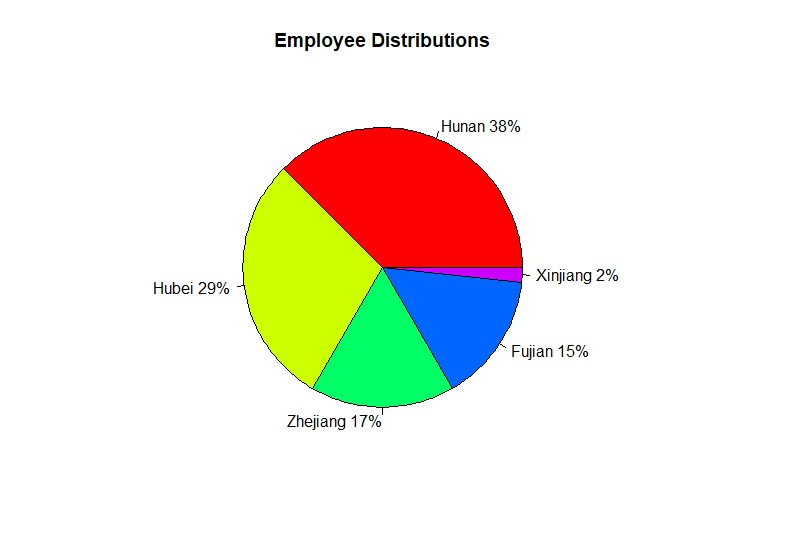
\includegraphics[width=1.2\textwidth]{Piechart.jpg}
\end{center}
According to the experiment results, most of the employees of the company come from Hunan province (38\%), and that the least employees come from Xinjiang ; The descending ranking of provinces in terms of employees distributions are Hunan, Hubei, Zhejiang, Fujian, Xinjiang.
\subsection*{Problem 2}

\begin{center}
	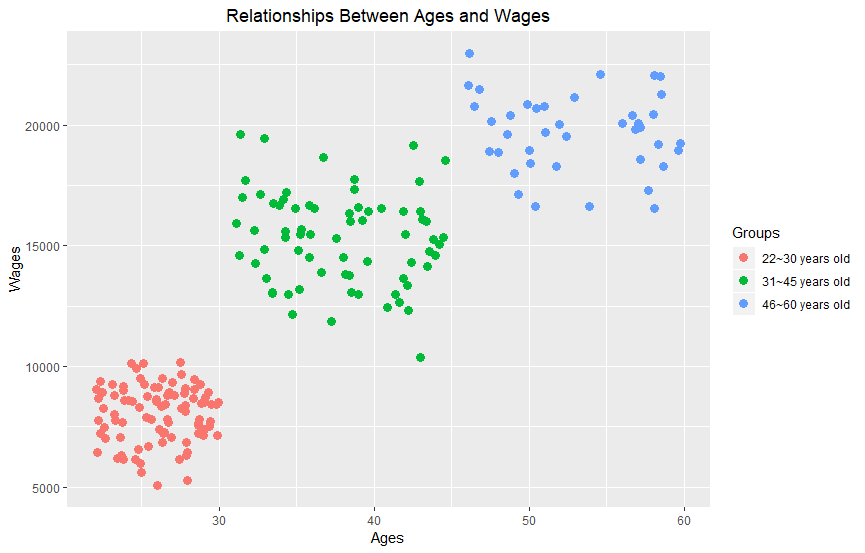
\includegraphics[width=1.2\textwidth]{Relationships.png}
\end{center}
According to the scatter plot, most of employees of 21-45 years old have wages of 7000-9000; most of employees of 31-45 years old have wages of 13000-17000; most of employees of 46-60 years old have wages of 18500-21500; wages of employees are positively propotional to their ages.
\subsection*{Problem 3}

\begin{center}
	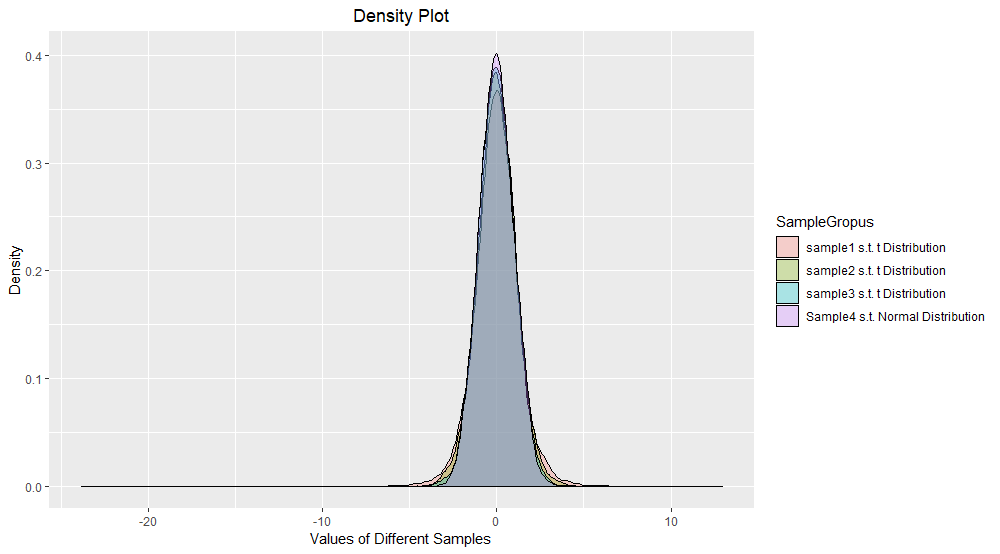
\includegraphics[width=1.2\textwidth]{Density.png}
\end{center}
According to the density plot, t distributions with smaller degree of freedom have lower peak and fatter tails; t distribution get close to normal distribution when degree of freedom gets greater.
\subsection*{Problem 4}
\begin{center}
	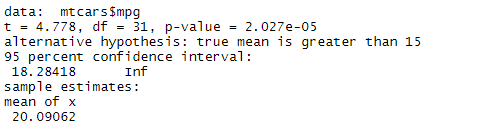
\includegraphics[]{p4.png}
\end{center}
Because we need to test whether the mean is larger than 15, we first construct a null hypothesis "The mean of mpg is less than or equals 15" \& alternative hypothesis "The mean of mpg is larger than 15". It is a single sample mean test, so we use t.test function to conduct hypothetical test  with $mu = 15$ and $alternative == greater$. According to t statistics of 4.778 and p-value of 2.023e-05, null hypothesis is rejected at significance level of 0.05. we accept that mean of mpg (miles per gallon) is larger than 15.
\subsection*{Problem 5}

\begin{center}
	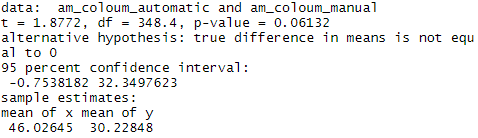
\includegraphics[]{p5.png}
\end{center}
Because we need to test whether the means of weights of cars are different in the automatic and manual, we first make the null hypothesis "means of weight of automatic and manual cars are equal" \& alternative hypothesis "means of weight of automatic and manual cars are different". It is a two sample mean test, so we use t.test function to conduct hypothetical test with $alternative == two-sided$. According to t statistics of 1.8772 and p-value of 0.06132, null hypothesis cannot be rejected at significance level of 0.05. We can accept that  wt (weight) of the cars are equal in the automatic and manual.

\subsection*{Problem 6}

\begin{center}
	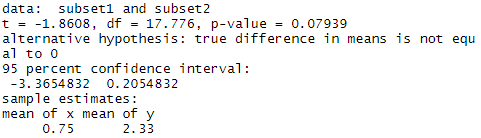
\includegraphics[]{p6.png}
\end{center}
Because we need to test whether the two drugs have similar effects, we first make the null hypothesis that "the mean effects of the two drugs are equal" \& alternative hypothesis "the mean effects of the two drugs are different". It is a two sample mean test, so we use t.test function to conduct hypothetical test with $alternative == two-sided$. According to t statistics of -1.8608 and p-value of 0.07939, null hypothesis cannot be rejected at significance level of 0.05. We accept that the two drugs have similar effects.

\end{document}